\documentclass {article}
\usepackage{fullpage}
\usepackage{forest}
\usepackage{graphicx}
\usepackage{courier}

\begin{document}

\begin{center}
\Large
$ $
\newline
\newline
\newline
\newline
\newline
\newline
\newline
\newline
\newline
\newline
\newline
\newline

Final Project Report

\textbf{3D Open World}

Name: Eric Bonn

Student ID: 20462900

User ID: eaibonn
\pagebreak

\tableofcontents

\end{center}
\vfill ~\vfill~
\newpage

\clearpage

\section{Project Information and Goals}

\subsection{Purpose}
    The purpose of this project is to build a 3D explorable world. The 3D world will be explorable via a 3D humanoid model that the user can control.

\subsection{Topics and Goals}
    \subsubsection{Modelling}
    Modelling a scene is an important aspect of a 3D explorable world and the scene must be engaging and interesting for the user. This can be done in a large number of ways; in this project, cel shading and texture/bump mapping are utilized. Modelling an interesting world is the most important goal because it is the thing with which the user directly interacts.

    \subsubsection{Animation}
    It is all about creating an ideal user experience; animation is another component of this. The character model is the user's connection into the world, it should be believable. This includes animating and adding sound.

    \subsubsection{Texture Mapping/Bump Mapping}
    Texture and bump mapping are methods to make the world seem more real, and more interesting. Texture mapping is able to bring to life objects that would otherwise seem very flat looking and bump mapping enhances this further.

    \subsubsection{Physics and Collision}
    Physics and collision are both required to make the 3D world as realistic as possible.

\subsection{Objectives}

\begin{enumerate}
     \item[1.]  Modelling the scene

     \item[2.]  User Interface

     \item[3.]  Keyframe Animation using linear interpolation

     \item[4.]  Sounds synced to model's running animation

     \item[5.]  Textures

     \item[6.]  Bump Mapping \textbf{[not implemented]}

     \item[7.]  Static Collision

     \item[8.]  Dynamic Collision

     \item[9.]  Cel Shading

     \item[10.]  A physics engine to support jumping

\end{enumerate}


\subsection{Statement}
The concept of an open world is an interesting one, and one that definitely interests me greatly. The possibility of creating something interesting and engaging that the user can be engrossed in is what intrigues me the most; it is one of the main reasons why I chose this as my project. This is also one of the primary focuses (creating an engaging, engrossing, interesting world) of the gaming industry, and although it isn't an industry that I necessarily want to have a career in, it is a industry that interests me. The gaming widely uses texture mapping, bump mapping, physics nd animation to create the greatest possible experience for the users. Often times cel shading is used to create an interesting aesthetic in games (see: Legend of Zelda Wind Waker) and that is one of the reasons why I wanted to incorporate cel shading into this 3D world.
\newline
\newline
Not only did I want to incorporate cel shading into the 3D world, texture mapping, bump mapping, animation, physics, collision, sounds, and of course a UI, were all necessary. All of these were chosen with one goal in mind: making an engaging, engrossing, and interesting world. As stated above, the cel shading was chosen to create a particular aesthetic that I found interesting, one that I had seen in such games as Legend of Zelda: Wind Waker. Texture mapping can be used to improve the quality of objects in the world, making them seem less flat, and bump mapping can enhance this further by adding more depth. Animations is of course necessary in any open world, especially one with a controllable character. The controllable character must have a walk animation, because if it doesn't the world will seem unbelievable and much less interesting. And what is a world without sound? So sounds must also be incorporated in various forms; environment sounds and more importantly movement sounds are beneficial to creating an interesting and realistic world. In that same vein, collision detection (both static and dynamic) adds realism to the world. If there was no collision detection and the user could move the character anywhere and everywhere, well that wouldn't be very interesting. If there's one thing I've learned from open world video games and MMORPGs, it's that people really like to jump; it can make walking more interesting (you can jump while you walk, giving you something to do), and gives an additional action for the user to perform on the character, thus adding depth. For these reasons a physics engine was necessary, so that when the character jumps it would abide by the laws of physics and follow a reasonable trajectory path, based on launch angle and speed. Finally, any and every game needs some sort of UI, so it is a given that this will be utilized.
\newline
\newline
The user interface includes all user interaction, from the user input to move the character to the menu bar on the screen. Here is a list of all the user interface components in this 3D world:\\
1. Quit button\\
2. Hide Menu\\
3. FPS\\
4. Game Time\\
5. Character movement\\
6. Character jumping\\
7. Camera movement\\
8. Toggle for Texture Mapping\\
9. Toggle for Bump Mapping\\
10. Toggle for Cel Shading\\
\newline
For details about these interface components, and how to use them, see the interaction component of the Project Manual.
\newline
\newline
From this project I hoped to learn more about making an interesting and engaging world. I wanted to learn more about animation, texture mapping, bump mapping and other techniques for creating such a world, and I believe I achieved this.\\
\newpage
\subsection{Milestones}
Order is important when it comes to implementing the 3D world. This is a list of the milestones I planned to achieve prior to starting the project, and the order with which I planned to achieve them. Modelling the scene is the most crucial because without a scene there is no way to verify or test any other features, so completing that first was paramount. In the case of the bump mapping milestone, I had to forfeit its completion in exchange for fully completing the UI and the world (and all the final details). 
\newline
\newline
\indent1. Create a basic world that I can test objectives in\\
\indent2. Create the character model, implement movement of the character model and \newline
\indent \indent camera (which follows the character model) \\
\indent3. Create running animation of the character \\
\indent4. Sync sound up to the running animation of the character \\
\indent5. Static collision \\
\indent6. Create dynamic objects, and then complete dynamic collision. Sync sound up to dynamic objects. \\
\indent7. Build physics engine so the character can jump \\
\indent8. Texture mapping \\
\indent9. Cel Shading \\ 
\indent10. Bump mapping \textbf{[milestone incomplete]} \\ 
\indent11. Complete full scene, adding final touches and details \\
\indent12. Complete User Interface \\

\pagebreak

\section{Project Manual}

\subsection{Compiling and Running the 3D Open World}
Compile steps: (see also: README)\\
1. \texttt{premake4 gmake} at root \\
2. \texttt{make} at root \\
3. Go to World3D directory \\
4. \texttt{premake4 gmake} \\
5. \texttt{make} \\ \newline
The 3D Open World can be used in a similar way as assignment 3. When executing the compiled World3D source you must also have a Lua script as an input parameter. This lua script is used to render the world and the character. See Input under Communication Section for more details.

\subsection{Communication}
\subsubsection{Input}
See below the command for running the compiled World3D source.\\
\newline
\texttt{./World3D [lua-script]}\\
\newline
In place of [lua-script] should be the path to a valid Lua script representing the world and character that should be rendered.\\
For this project the world scene and character can be found in the \texttt{./World3D/Assets/World3D.lua}\\
So after compiling, to run the built world and character use the following command in the \texttt{World3D} directory:\\
\newline
\texttt{./World3D Assets/World3D.lua}\\
\newline
A valid lua script must have a root node with exactly two children. One child represents the puppet and this node must have the name "puppet", the second represents the entire world scene (static objects, dynamic objects, and so on) and this node must have the name "world". These two nodes can have as many children as necessary, the aforementioned restrictions are the only ones. See the tree below for a visualisation of the Lua script structure.
\newline
\newline
\begin{forest}
    [\texttt{root}
     [\texttt{puppet}
     []
     []
     []
     ]
     [\texttt{world}
     []
     []
     []
     ]
    ]
\end{forest}

\subsubsection{Interaction}
Upon inputting the script the application will begin and the user will be able to see the character from the back in the rendered world scene, and as was mentioned before the 3D world has a user interface for interaction. See below available commands in the 3D world:\\
1. Quit Button\\
\indent - Quit button in menu\\
\indent - shortcut Q\\
2. Hide Menu\\
\indent - shortcut M\\
3. Character movement\\
\indent - Arrow keys for moving/turning the character model(up/down/left/right)\\
\indent - camera will turn with the character, so it is always in the same position/orientation relative to the \indent character model\\
4. Character jumping\\
\indent - shortcut Spacebar\\
5. Camera movement\\
\indent - \texttt{CTRL +} Arrow keys for turning the camera (up/down/left/right)\\
\indent - camera will pivot (turn) around the character model\\
6. Toggle for Texture Mapping\\
\indent - shortcut T\\
7. Toggle for Bump Mapping\\
\indent - shortcut B\\
8. Toggle for Cel Shading\\
\indent - shortcut C\\

\subsubsection{Output}
The output of running the application with the Lua script will be the rendered interactible character and scene. Performing any of the above actions will of course result in that action being the output (arrows move the character, Q quits etc.)\\
The image below is a screenshot of running World3D with the built Lua Script, \texttt{Assets/World3D.lua}\\
\newline

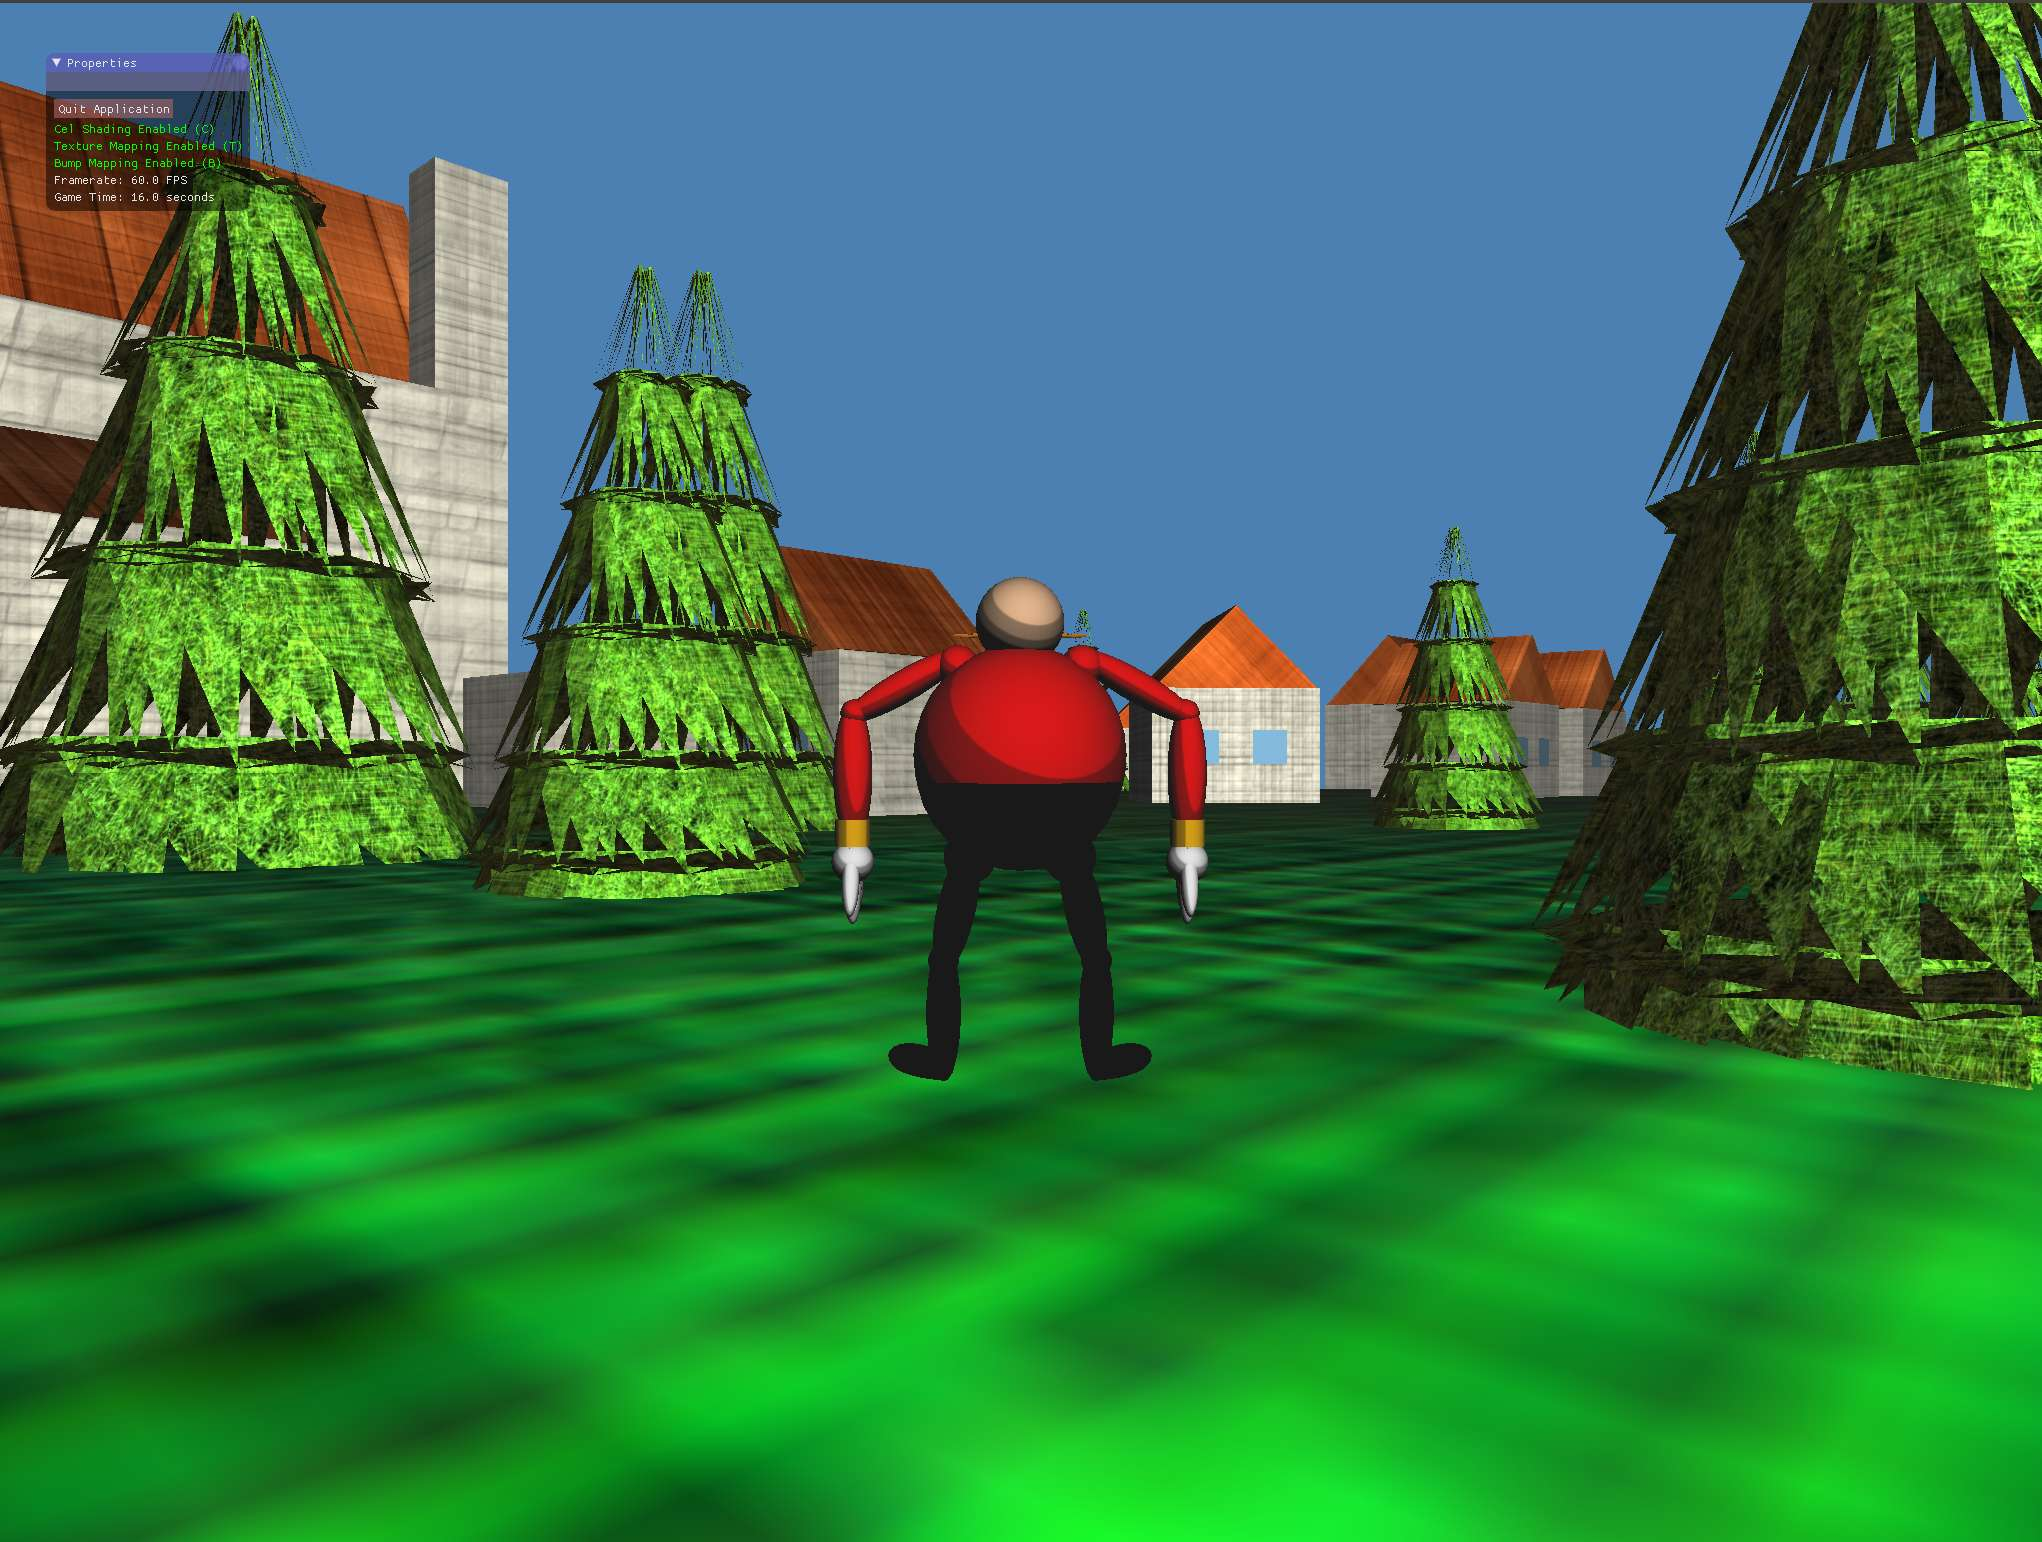
\includegraphics[width=100mm]{screenshot.jpg}

\pagebreak

\section{Code Organization}
\subsection{File Structure}
All necessary files are located in the submitted Project.zip\\ \newline 
All library archive files for SOIL, GLFW etc. can be found in \texttt{lib/}.\\ \newline
\texttt{premake4.lua} will generate a \texttt{Makefile} which can then be run to update anything in the library.\\ \newline
All shared source files and headers can be found \texttt{shared/} . This includes the source files for SOIL, GLFW etc.\\ \newline
The source code for the project can be found under \texttt{World3D/}\\ 
All source files have the extension \texttt{*.cpp} and all header files have the extension \texttt{*.hpp}\\
Two sound files in the form \texttt{.wav} can be found in the \texttt{World3D/} directory.\\ \newline
Simarly, there is a \texttt{premake4.lua} script in the directory that will create the \texttt{Makefile}\\ \newline
In \texttt{World3D/Assets/} there are all the Lua scripts and \texttt{.obj} files. The \texttt{.obj} files are the object files used in the Lua scripts, including the world Lua script for this project. The world scene script can be found in this directory: \texttt{World3D/Assets/World3D.lua} \\ \newline
Texture images and normal maps can be found in \texttt{World3D/Textures/}

\subsection{Code Outline}
A high-level overview of code on a file-by-file basis:

\subsubsection{Character.cpp/hpp}
Contains the definition and implementation of the \texttt{Character} class. This class is responsible for holding the character keyframes for the animation, and performing the jump/run animations.

\subsubsection{DynamicObject.cpp/hpp}
Contains the definition and implementation of the \texttt{DynamicObject} class. This class is responsible for movement of the object (hence it being dynamic) and also contains other information about the object, for instance its direction of movement, the speed its moving and its initial position.

\subsubsection{general.cpp/hpp}
Contains the definition and implementation for a couple general use functions, that are very useful and therefore used in several classes. This includes a getNode function, which traverses an arbitrary tree to find a specific SceneNode, and collided which simply takes two SceneNodes (representing two objects) and returns true if they collid.

\subsubsection{GeometryNode.cpp/hpp}
Contains the definition and implementation of the \texttt{GeometryNode} class. This class extends the \texttt{SceneNode} class (see SceneNode section), and represents a node in our render tree that is an object (ie. something that needs to be rendered). GeometryNodes are rendered in the World3D class based on the mesh ID and the material.

\subsubsection{JointNode.cpp/hpp}
Contains the definition and implementation of the \texttt{JointNode} class. This class extends the \texttt{SceneNode} class (see SceneNode section), and represents a joint in a puppet model. A JointNode is defined by rotation amounts and rotation ranges. JointNodes typically connect two GeometryNodes and allow for rotation between them.

\subsubsection{Main.cpp}
Contains the \texttt{main()}, which simply creates and instance of cs488 window (parent class of World3D).

\subsubsection{scene{\_}lua.cpp/hpp}
Contains the definition and implementation for the \texttt{import{\_}lua} function, which is used to import Lua script into World3D.

\subsubsection{SceneNode.cpp/hpp}
Contains the definition and implementation of the \texttt{SceneNode} class. This class represents a node in the render tree. A SceneNode is a general node and contains general information about the node in the tree, such as its bounding box (used for collision detection), as well as the transform matrix. SceneNode also has a list of its children (also SceneNodes) in the tree. SceneNode has transformation functions (rotate, translate, scale) that apply rotations etc. to not only that nodes matrix but also its children.

\subsubsection{Texture.cpp/hpp}
Contains the definition and implementation of the \texttt{Texture} class. This class is responsible for holding all the information required to initialize and bind a texture for use, including texture ID, texture path (directory path to the image), as well as width/height of said image. It has an \texttt{init()} function that is to be called upon instantiation which generates the texture ID, binds it, and sets the \texttt{glTexParameteri}

\subsubsection{World3D.cpp/hpp}
Contains the definition and implementation of the \texttt{World3D} class. This class contains all the information needed to render and run the world. The \texttt{World3D} class holds instances of \texttt{Character}, \texttt{Texture}, \texttt{DynamicObject}, as well as a couple \texttt{SceneNode} representing the puppet model and the world model. \texttt{World3D} is also responsible for a lot of the heavy lifting in the application, including performing collision detection, rendering, updating vertex buffer data, uploading uniforms to Vertex/Fragment Shader. In addition it also handles the GUI, event handling, and much of the app logic (such as \texttt{move()} functions) in the application.

\newpage

\section{Implementation}
\subsection{Modelling the Scene}
Modelling the scene involves creating the necessary Lua script (following the necessary structure) to pass as a parameter to the executable in order to create the render tree. The scene can be modelled using several commands, such as \texttt{gr.node, gr.mesh, gr.material, gr.joint} and more. \texttt{.obj} files can be used in the Lua scripts to create the shapes, cubes, spheres etc. In this project a couple of interesting \texttt{.obj} were used, including corn and trees. These objects are then represented by nodes in the render tree (GeometryNodes) which will be rendered accordingly to the data in the \texttt{.obj} as well as its material and/or texture.\\
\newline
Below is once again the structure of the render tree from the Lua script, with the root node of Lua script having the puppet and the world scene as its immediate children.
\newline
\newline
\begin{forest}
    [\texttt{root}
     [\texttt{puppet}
     []
     []
     []
     ]
     [\texttt{world}
     []
     []
     []
     ]
    ]
\end{forest}

\subsection{User Interface}
The user interface menu was completed using the ImGui library, which can be found in the \texttt{shared/imgui/} directory. ImGui allows for the creation of buttons, text, and menu windows. See below an image of the UI menu for this project:\\ \newline

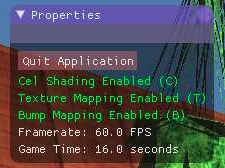
\includegraphics[width=50mm]{imgui.jpg}

$ $ \newline The code for the UI menu can be found in the \texttt{World3D} class in the \texttt{guiLogic()} function. In addition to ImGui UI in this project, there is also event handling for keyboard input. The input of the arrow keys for moving the character, the quit button, toggles etc. must all be handled. This is also done in the \texttt{World3D} class, but in the \texttt{keyInputEvent} function.

\subsection{Keyframe Animation using Linear Interpolation}
Animation is done primarily on the Character model, so all the animation code lives in the \texttt{Character} class, including the \texttt{KeyFrame} struct.
\subsubsection{Keyframes}
A \texttt{KeyFrame} struct was created in \texttt{Character.hpp} to hold all the information contained within a Keyframe. In this project, a Keyframe is defined as a rotation amount on specific joints on the character model. Following this structure, a single Keyframe can be various rotations on various joints. For instance, in this project, one KeyFrame does rotation on the leftShoulderJoint, rightShoulderJoint, leftHipJoint, and rightHipJoint.\\
All Keyframes are defined in \texttt{initKeyFrames()} in \texttt{Character}. Linear interpolation is then done on these Keyframes to get the smoothness in the animation

\subsubsection{Linear Interpolation}
To create the smoothness in animation, we use linear interpolation. This involves calculating a step amount in between two Keyframes, and then at each iteration between those two Keyframes, increase by that step amount.\\ \newline
First we define the amount of steps that we want to interpolate between Keyframes, \texttt{INTERPOLATION{\_}STEP{\_}SIZE} \\ 
To then get the step amount between the two Keyframes: \\ \newline
$StepAmount = \frac{keyframe_i - keyframe_{i-1}}{INTERPOLATION{\_}STEP{\_}SIZE}$ \\ \newline
Note: the step amount represents a rotation of a joint in this definition of a Keyframe, and the above arithmetic is done purely between numbers (Keyframe rotation amounts). So then once we have this step amount, we add this amount to that joint's rotation at every iteration in between those two Keyframes. Once we reach the next Keyframe however, the step amount is recalculated. [4][5]\\
This code can be found in the \texttt{runAnimation()} function in \texttt{Character} 

\subsection{Sound}
To sync sound to the model animation, I played a \texttt{.wav} (which can be found in \texttt{World3D} directory) at a specific frame. This is done using the C++ \texttt{system()} command, as well as Linux's \texttt{canberra-gtk-play}. I added an \& at the end of the command to ensure it runs in the background \\ \newline
Full command example: \\
\texttt{system("canberra-gtk-play -f step{\_}grass.wav \&");} \\ \newline
Can be found in \texttt{runAnimation()} in \texttt{Character}

\subsection{Texture Mapping}
To implement texture mapping in OpenGL, a texture ID must first be generated, then bound, and using SOIL the image is retrieved. Next, the texture parameters are set and the MIP map is generated. This is done when the texture is first initialized, \texttt{init()} in the \texttt{Texture} class. After the initialization parameters are all set, and the texture ID generated, the texture ID must simply be rebound to be used again. What determines the texture that is bound depends on the type of object. By type of object I mean, roof, building, grass, soil etc, which is determined and set in the Lua script. The object type is checked in \texttt{World3D} when shader uniforms are being updated, and then the appropriate texture is bound accordingly.\\ \newline
On the FragmentShader side of things, with the texture now bound to a uniform Sampler2D, the Shader can grab the colour of the texture at position UV, and then incorporate that colour when determining the colour for that pixel (ie. the FragColour). This can be done using the texture mapping function \texttt{texture} with the bound texture and the UV in the x, y, and z directions. [2]

\subsection{Bump Mapping}
Bump mapping is implemented in a similar way to texture mapping. In my implementation, a bump mapping object is treated the same as a texture mapping object, that is to say they both use the \texttt{Texture} class and the \texttt{init()} function. Similarly, bump maps are bound in the same way as texture maps in the \texttt{World3D} uniform function. However,  Bump mapping does not use a regular image, but rather it uses a normal map in image format. The normal map is a represenation of all the heights/shadows of the texture, the normal map in conjunction with the texture map enhances the object and makes it look much more realistic.\\ \newline
The main difference in Bump mapping and Texture mapping lies on the FragementShader side of things. In the texture mapping you simply grab the colour of texture at the UV coordinate, and incorporate that into the FragColour, but in bump mapping, you use the colour/depth of the normal map to create a new normal. This new normal will be used in the Phong Shading instead of the old normal of the surface (the one calculated for the whole object/face). This normal with the Phong Shading Model will then create the illusion that there is a bump there because of the shadows/shading. If a normal map of a texture is used over top of said texture (ie. bump mapping and texture mapping are used), then the texture will appear to have more depth. [2]

\subsection{Static Collision}
Static collision is done by creating bounding boxes for every single object in the world, including the character. The \texttt{BoundingBox} structure lives in \texttt{SceneNode.hpp}. These bounding boxes are initialized to the same 1x1x1 cube when the SceneNode is initialized, but they are then subjected to the same transformations as the SceneNode transformation matrix. The structure contains the minimum point of the bounding box and the maximum point. So all scaling, translating, and rotating also occurs to this bounding box. When it comes to the actual static collision detection, at any given iteration, check to see if any dynamic objects (character etc.) are colliding with a static object. Collision is detected with the \texttt{collided()} function in \texttt{general.cpp} and it compares it in the following way:\\
\indent 1. Translate object1 and object2 back to the origin2\\
\indent 2. Translate object1 the distance it was from object2 prior to the initial translating\\
\indent 3. Rotate both objects back to their initial orientation\\
\indent 4. Check to see if any part of object1 is inside of object2\\ \newline
\indent \indent \texttt{object1.min > object2.min and object1.min < object2.max or}\\
\indent \indent \texttt{object1.max > object2.min and object1.max < object2.max}\\ \newline
If this above inequality is satisfied then that means part of object1 lies in object2 so they've collided, and therefore indicate as such. The dynamic object cannot move forward while it is colliding. And if it is the character controlled model that is colliding then it will simply run in place. \\ \newline
In addition to there being collision code in \texttt{general.cpp} there is also collision code in \texttt{World3D} in the \texttt{checkCollision()} function.\\ \newline
Efficiency is very important when it comes to collision detection because it can very easily be come too slow, especially if the collision detection is doing some heavy calculations. It is for this reason that some efficiency measures must be put in place. To avoid the collision detection comparing every single dynamic object with every single static object at every iteration, check first to see if the two objects are within a certain threshold, if they aren't even within this set threshold, don't even bother comparing them. This ends up sparing a lot of a what would be unnecessary calculations because dynamic objects don't have to compare with every object in the whole world. [1]
\newpage
\subsection{Dynamic Collision}
Dynamic collision works the same as static collision except between two dynamic objects, instead of a dynamic object an a static object. The two dynamic objects are checked for collision in the same way as a dynamic and static objects are checked, using the \texttt{collided()} function in \texttt{general.cpp}. \\ \newline
A differing point in dynamic and static collision is that dynamic collision requires a sort of \textit{reaction} from the objects upon collision. Whereas with static collision, the dynamic object can just not move during a collision, that doesn't necessarily make as much sense with dynamic objects (that they stop moving), depending on what directions they collide. For dynamic collision detection in this project I have two main cases, colliding while moving in the same direction and colliding while moving in opposite directions. For the same direction, the character model collides and simply cannot move any further. However, if they are moving in the opposite direction (or the dynamic object hits the character or another object while it is still) then the dynamic will switch direction and begin going back the other way. \\ \newline
Similar to static collision, efficiency is very important to dynamic collision. Because of this it was necessary to make the same threshold checks between dynamic objects, in order to reduce unnecessary collision checks. [1]

\subsection{Cel Shading}
Cel Shading (or toon shading) is a type of shading that creates a different aesthetic; a more cartoony look than other traditional shading methods. This is done by dividing shaded areas into groups based on thresholds, and then filling that area with a single shade. This is done by first defining thresholds between 0 and 1 (representing the percentage of light), and then shadow found in a certain range will be clamped down. This creates the below effect. On the left is the cel shading on puppet in the world, on the right is an example of cel shading on a teapot. Note the solid shaded areas in both cel shaded objects. [3]\\ \newline

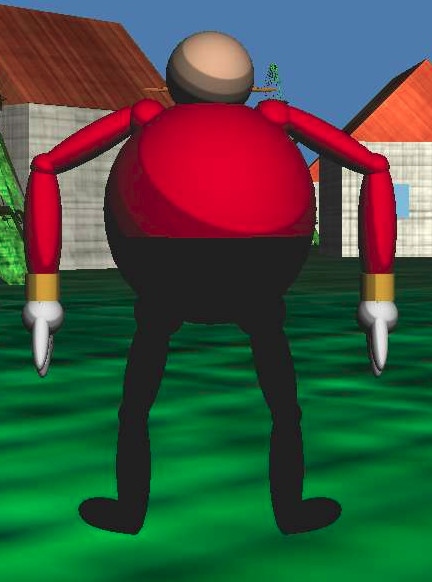
\includegraphics[width=50mm]{celshadedmodel.jpg}
\indent \indent 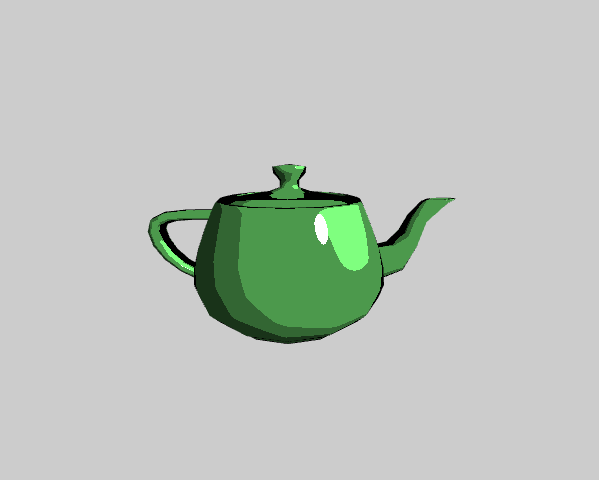
\includegraphics[width=80mm]{toonpot.png} \\ \newline
Cel shading is achieved by modifying the FragmentShader and how it determines the final FragColour. In order to achieve the clamped shading, only a percentage of diffuse shading and specular shading must be used. Depending on which range (between thresholds) the diffuse factor lies, determines what percentage of it will be used (ie. how much it will be clamped down). In order to create smooth and crisp shading in between the areas, \texttt{smoothstep/step} functions should be used to interpolate specular factors (hermite interpolation)

\subsection{Physics Engine}
When implementing the physics engine, established and known physics formulas were used. Below is a formula to calculate the height at a given $x$ value on the trajectory path.\\ \newline
$y = y_0 + x \tan \theta - \frac {gx^2}{2(v\cos\theta)^2}$\\ \newline
Using this formula, the height corresponding to any $x$ value can be found.\\
The character model has constant speed whenever it is walking, so upon hitting the spacebar the character will always have the same defined speed. In terms of angle it is always $\theta = 45^{\circ}$\\
Gravity is of course g, $g = -9.8$\\
The $x$ value is equal to what the $x$ value is on the iteration that we're checking. So the way the physics engine works altogether, is when the user hits the spacebar the character model is deemed to be midair (\texttt{midair=true}), and the values are all initialized and calculations begin at this point. Using \newline \texttt{calculateTrajectoryHeight()} in \texttt{World3D}, the $x$ value at that iteration is passed and the height the character model should have is then calculated, the model is then translated to that height. This goes on (and the model stays in air) until \texttt{modelheight < groundheight}, at which point the height calculations stop and the character model is considered no longer in midair, \texttt{midair=false}

\newpage
\section{Conclusion}
I have learned a lot throughout this project, but perhaps the most important thing is the realization that there is a lot of time and hardwork that goes into making highly detailed, realistic, interesting and engaging 3D worlds. Calculations must all be efficient and done only when necessary in order to better improve performance because it is very very easy for performance to become bad very very quickly by simply ignoring efficiency. A lot of the calculations are done many times a second, and so a time save anywhere can actually save a lot of time, and the inverse of that: one small repeated unnecessary calculation can slow down performance. Overall the project was a good experience.

\newpage

\section{Bibliography}

[1] Watt, A and Policarpo, F {\it 3D Games: Real-time rendering and software technology} Addison-Wesley, 2001, Chapter 15\\\relax
\\\relax
[2] Watt, A and Policarpo, F {\it 3D Games: Real-time rendering and software technology} Addison-Wesley, 2001, [pp. 224-228]\\\relax
\\\relax
[3] Pascal Barla, Joelle Thollot {\it X-Toon: An Extended Toon Shader}, University of Michigan, https://hal.inria.fr/inria-00362888/file/x-toon.pdf \\\relax
\\\relax
[4] School of Computer Science, University of Waterloo {\it CS488/688 - Introduction to Computer Graphics} [pages 247 to 248] Waterloo, Winter 2016\\\relax \newline
[5] School of Computer Science, University of Waterloo {\it CS488/688 - Introduction to Computer Graphics} In-Class Lecture, Mar 22, Waterloo, Winter 2016

% Delete % at start of next line if this is a ray tracing project
% A4 extra objective:
\end{document}
